%Ich bin ein TeX Dokument
\documentclass{scrartcl} % KOMA-Script Dokumentenklasse Article
%Für Positionierung von Gleitumgebungen
\usepackage{scrhack}
% Warnung, falls noch einmal kompiliert werden muss
\usepackage[aux]{rerunfilecheck}
% Paket für Schriftarteinstellung, muss immer geladen werden
\usepackage{fontspec}
% Deutsche Spracheinstellungen, wichtig z. B. für korrekte Trennung
\usepackage[ngerman]{babel}
% mehr Pakete hier
\usepackage{amsmath}
\usepackage{amssymb}
\usepackage{mathtools}
%ISO Normen benutzen
\usepackage[
math-style=ISO,
bold-style=ISO,
sans-style=italic,
nabla=upright,
partial=upright,
]{unicode-math}
%Für korrekte Zahlen mit Einheiten
\usepackage[
locale=DE,
separate-uncertainty=true,
per-mode=symbol-or-fraction,
]{siunitx}
% Unterstützung für Links und PDF Metadaten
\usepackage[unicode]{hyperref}
\usepackage{bookmark}
%Für das Einbinden von Grafiken
\usepackage{graphicx}
%Positionierung von Gleitumgebungen
\usepackage{float}
%Für Tabellen
\usepackage{booktabs}
% Einstellungen hier, z.B. Fonts
\setmathfont{Latin Modern Math}
\floatplacement{figure}{H}
\floatplacement{table}{H}

\begin{document}
\title{Versuch D206 "Die Wärmepumpe"}
\author{Henry Krämerkämper \and Christopher Breitfeld}
\date{29.10.2020}
\maketitle
\newpage
\tableofcontents
\newpage
\section{Einleitung}
Der Versuch "Die Wärmepumpe", welcher im Folgenden erklärt und durchgeführt wird, behandelt den Transport von
Wärmeenergie von einem kälteren zu einem wärmeren Reservoir. Nach dem zweiten Hauptsatz der Thermodynamik sind beide
Flussrichtungen möglich, nur ist für den Transport vom kälteren zum wärmeren Reservoir zusätzliche Arbeit nötig. Diese verrichtet die Wärmepumpe.
Im Folgenden werden Merkmale dieser behandelt, in etwa die Güteziffer der Pumpe sowie ihr Massendurchsatz und der Wirkungsgrad des Kompressors.
\section{Theoretische Grundlagen}
Im Folgenden wird immer der Differentialquotient anstelle des Differenzenquotienten verwendet, da alle Berechnungen auf einer nicht-linearen Ausgleichsrechnung fußen.
  \subsection{Die Güteziffer}
  \label{sec:güteziffer}
  Die hier verwendete Wärmepumpe wird unter anderem durch die Güteziffer $ v $ charakterisiert. Sie gibt das Verhältnis zwischen der aufgewendeten Arbeit für den Wärmetransport
  $ A $ und der transportierten Wärmeenergie $ Q_\text{transp} $ an. Eine Formel für die Berechnung der Güteziffer lässt sich wie folgt herleiten: \\
  \\
  Wir bezeichnen die dem wärmeren Reservoir 1 zugeführte Wärmeenergie als $ Q_\text{1} $, sowie die dem kälteren Reservoir 2 entnommene Wärmeenergie als $ Q_\text{2} $.
  Dann gilt nach dem ersten Hauptsatz der Thermodynamik
  \begin{equation}
    Q_\text{1} = Q_\text{2} + A.
    \label{eqn:wärmeenergie1}
  \end{equation}
  Dann ist das Verhältnis zwischen transportierter Wärmeenergie und aufgewendeter Arbeit
  \begin{equation}
    \frac{Q_\text{1}}{A} = v.
    \label{eqn:güteziffer}
  \end{equation}
  Um die Güteziffer einer idealen Wärmepumpe zu berechnen, betrachten wir die Zusammenhänge nach dem zweiten Hauptsatz der Thermodynamik:
  %Finde ich persönlich schwach formuliert, hier müsste nochmal nachgearbeitet werden
  \begin{equation}
    \frac{Q_\text{1}}{T_\text{1}} - \frac{Q_\text{2}}{T_\text{2}} = 0
    \label{eqn:wärmeenergie2}
  \end{equation}
  Gleichung \eqref{eqn:wärmeenergie2} gilt nur unter der Vorraussetzung, dass der Prozess reversibel abläuft.
  Da dies in der Realität nicht möglich ist, muss \eqref{eqn:wärmeenergie2} im Falle eines irreversiblen Prozesses
  anders formuliert werden:
  \begin{equation}
  	\frac{Q_\text{1}}{T_\text{1}} - \frac{Q_\text{2}}{T_\text{2}} > 0
  	\label{eqn:wärmeenergie3}
  \end{equation}
	Aus Gleichung \eqref{eqn:wärmeenergie1} und Gleichung \eqref{eqn:wärmeenergie3}, sowie der Definition der Güteziffer
	\eqref{eqn:güteziffer}, ergibt sich die Güteziffer einer idealen Wärmepumpe zu
	\begin{equation}
		v_\text{ideal} = \frac{Q_\text{1}}{A} = \frac{T_\text{1}}{T_\text{1} - T_\text{2}}
		\label{eqn:idealegüteziffer}
	\end{equation}
	Dann gilt analog zu \eqref{eqn:idealegüteziffer} für die reale Güteziffer:
	\begin{equation}
		v_\text{real} < \frac{T_\text{1}}{T_\text{1}-T_\text{2}}
		\label{eqn:realegüteziffer1}
	\end{equation}
  Die reale Güteziffer lässt sich auch aus dem Differentialquotienten $ \frac{\increment T_\text{1}}{\increment t}$ berechnen. Die transportierte Wärmemenge $\increment Q_\text{1}$
  für ein Zeitintervall $\increment t$ ist dann:
  \begin{equation}
    \frac{\increment Q_\text{1}}{\increment t} = (m_\text{1}c_\text{w} + m_\text{k}c_\text{k}) \frac{\increment T_\text{1}}{\increment t}.
    \label{eqn:realegüteziffer2}
  \end{equation}
  Hierbei ist $m_\text{1}c_\text{w}$ die mittlere Wärmekapazität des Wassers in Reservoir 1 und $m_\text{k}c_\text{k}$ die mittlere Wärmekapazität der Kupferschlange und des Eimers.
  Für die reale Güteziffer $v_\text{real}$ gilt
  \begin{equation}
    v_\text{real} = \frac{\increment Q_\text{1}}{\increment t \cdot N}.
  \end{equation}
  Hierbei ist $N$ die Leistungsaufnahme des Kompressors über $\increment t$. Daraus folgt dann
  \begin{equation}
    v_\text{real} = (m_\text{1}c_\text{w} + m_\text{k}c_\text{k}) \frac{\increment T_\text{1}}{\increment t} \cdot \frac{1}{N}.
    \label{eqn:realegüteziffer3}
  \end{equation}
	An \eqref{eqn:idealegüteziffer} und \eqref{eqn:realegüteziffer1} kann man ablesen, dass eine Wärmepumpe eine höhere Güte hat,
	wenn der Temperaturunterschied zwischen Reservoir 1 und Reservoir 2 möglichst gering ist. Das bedeutet, dass der Engeriverlust
	für geringe Temperaturunterschiede am kleinsten ist.
	\subsection{Der Massendurchsatz}
	Der Massendurchsatz einer Wärmepumpe beschreibt, wie viel Wärme aus dem kälteren Reservoir 2 pro Zeiteinheit entnommen wird. \\
	Mitlhilfe des gemessenen Differenzenquotienten $ \frac{\increment T_\text{2}}{\increment t}$ sowie der Wärmekapazität von Reservoir 2
	$m_\text{2}c_\text{w}$ und der Wärmekapazität der Kupferschlange und des Eimers $m_\text{k}c_\text{k}$ ergibt sich der Massendurchsatz
	zu
	\begin{equation}
		\frac{\increment Q_\text{2}}{\increment t} = (m_\text{2} c_\text{w} + m_\text{k} c_\text{k}) \frac{\increment T_\text{2}}{t}.
		\label{eqn:massendurchsatz1}
	\end{equation}
	Da der Wärmetransport über Verdampfung eines Mediums stattfindet, kann man \eqref{eqn:massendurchsatz1} auch mithilfe der
	Verdampfungswärme $L$ schreiben:
	\begin{equation}
		\frac{\increment Q_\text{2}}{\increment t} = L \cdot \frac{\increment m}{\increment t}
		\label{eqn:massendurchsatz2}
	\end{equation}
  \subsection{Die mechanische Kompressorleistung}
  Für die verrichtete Arbeit $A_\text{m}$, die der Kompressor bei einer Volumenänderung von $V_\text{a}$ auf $V_\text{b}$ leistet, gilt
  \begin{equation}
    A_\text{m} = -\int_{V_\text{a}}^{V_\text{b}} p \symup{d}V.
  \label{eqn:arbeitkompressor}
  \end{equation}
  Dann ist die Leistung des Kompressors
  \begin{equation}
    N_\text{mech} = \frac{\symup{d} A_\text{m}}{\symup{d} t}.
    \label{eqn:leistungkompressor1}
  \end{equation}
  Unter der Annahme, dass die Kompression ein annähernd adiabatisch ablaufender Vorgang ist, und unter Verwendung der Poissonschen Gleichung erhählt man für $N_\text{mech}$
  \begin{equation}
    N_\text{mech} = \frac{1}{\kappa - 1}  \left(p_\text{2} \sqrt[\kappa]{\frac{p_\text{1}}{p_\text{2}}} - p_\text{1} \right)  \frac{\increment V_\text{a}}{\increment t}.
    \label{eqn:leistungkompressor2}
  \end{equation}
\section{Aufbau des Experiments}
    \subsection{Funktionsweise einer Wärmepumpe}
      Über ein Transportmedium, welches duch Verdampfung und Kondensation Wärme ab- oder aufnimmt,
      wird in Form von Phasenumwandlungsenergie Wärme aus Reservoir 2 in Reservoir 1 abgegeben.
      \begin{figure}
        \centering
        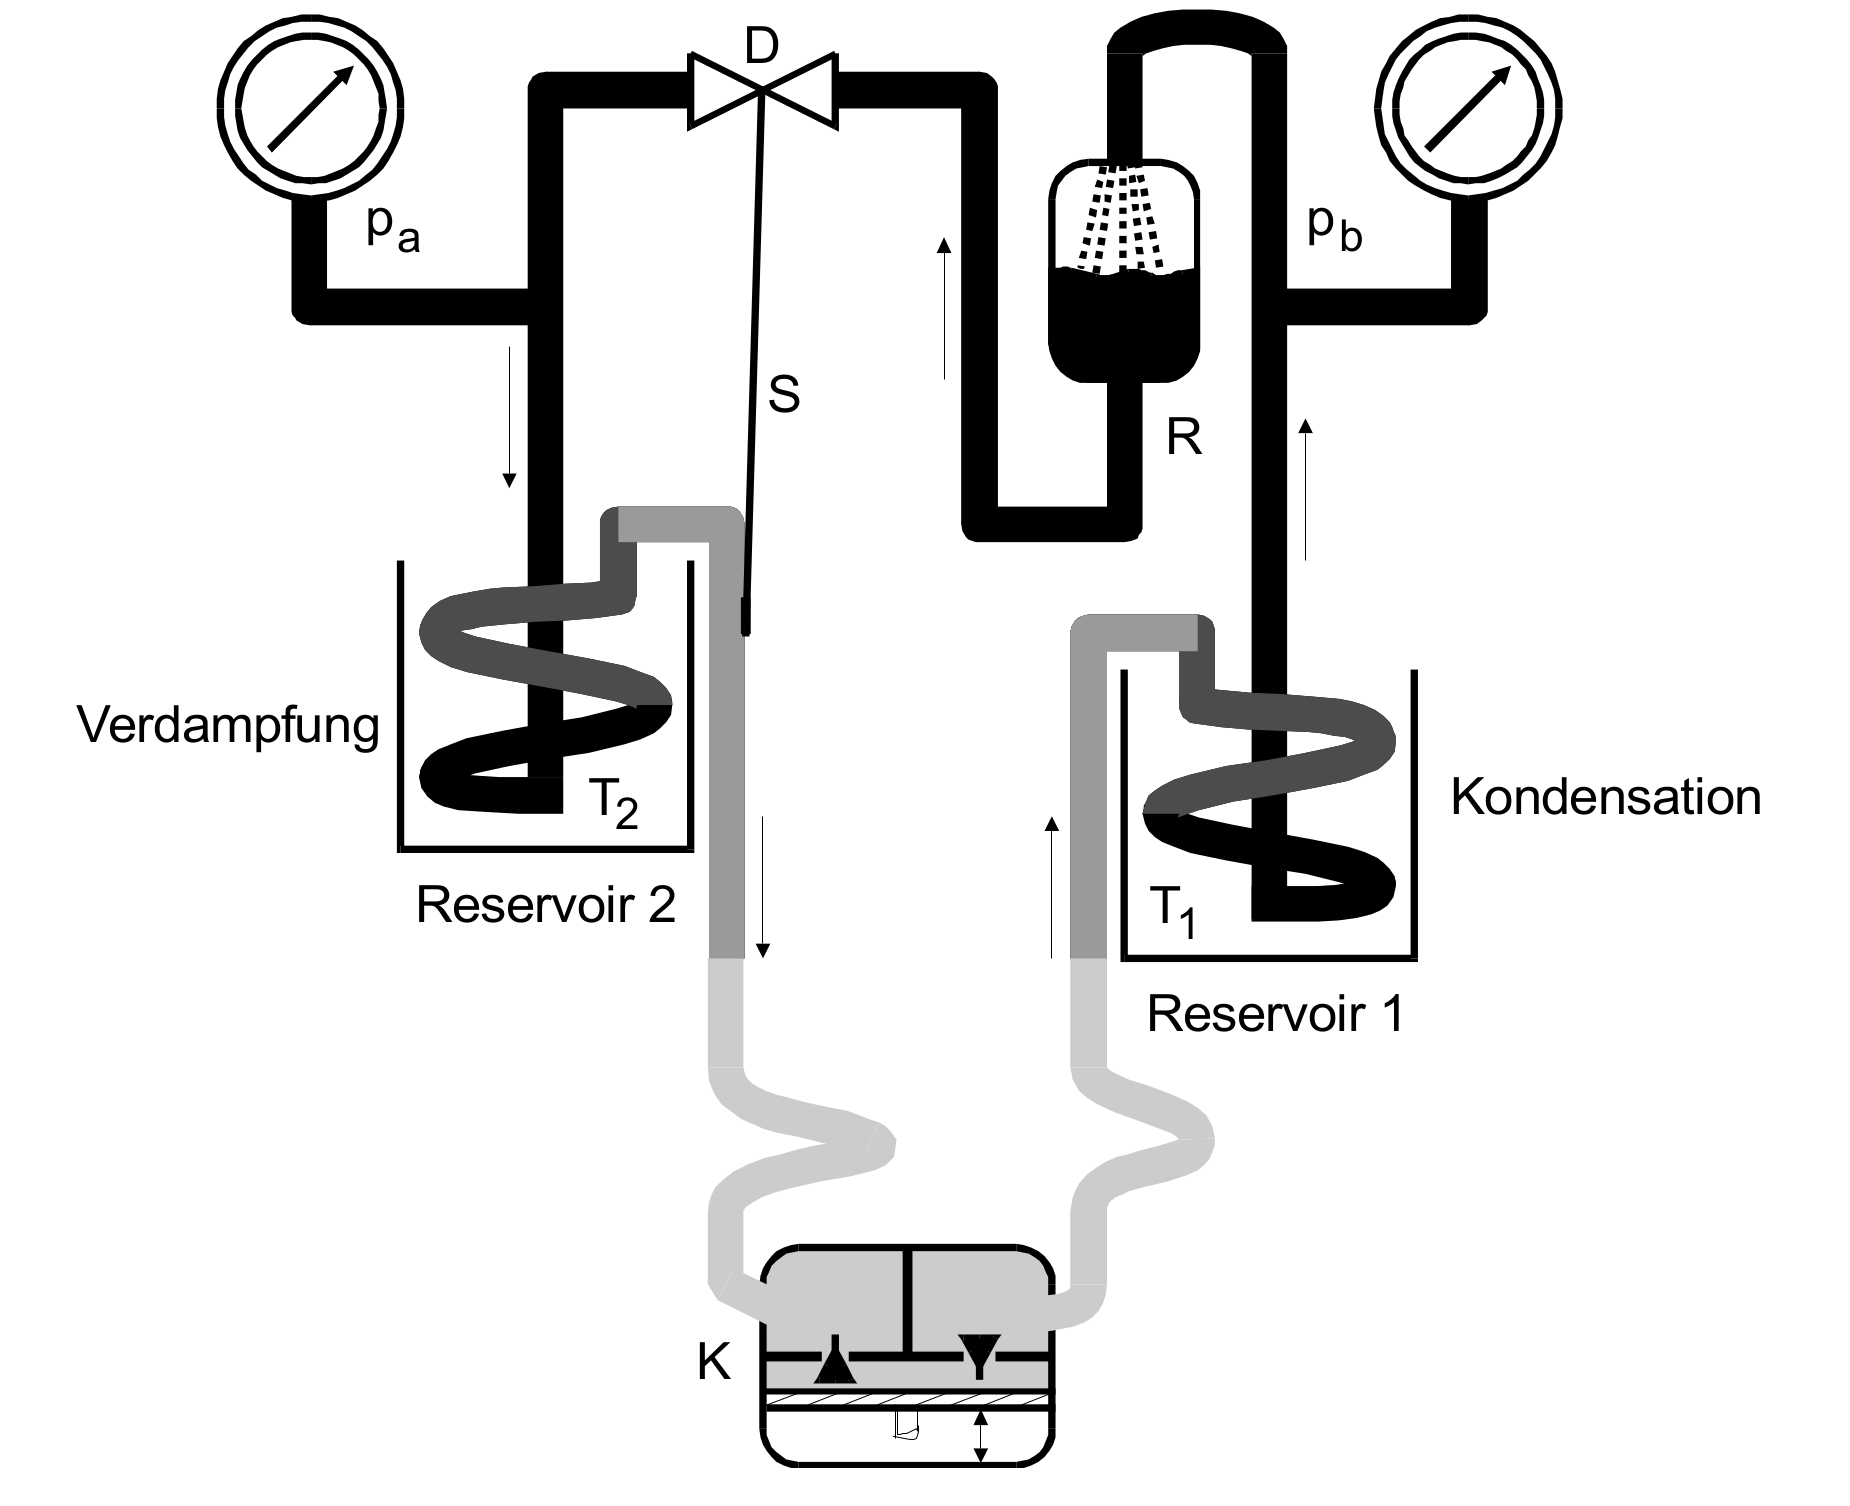
\includegraphics[scale = 0.15]{AufbauWaermepumpe.png}
        \caption{Schematische Darstellung einer Wärmepumpe.}
        \label{fig:wärmepumpe1}
      \end{figure}
      In Abbildung \ref{fig:wärmepumpe1} stellen die schwarz eingefärbten Leitungen den Abschnitt dar, in welchem das Transportmedium flüssig ist.
      Aus Reservoir 1 heraus fließt das Transportmedium mit Druck $p_\text{2}$ hinein in den Reiniger R, von wo aus dem Transportmedium alle Gasreste entfernt werden.
      Das gereinigte Medium gelangt durch das Drosselventil D. Durch den Strömungswiderstand des Ventils ändert sich der Druck auf $p_\text{1}$. Da das Medium bei Druck $p_\text{2}$
      flüssig, bei Druck $p_\text{1}$ jedoch gasförmig ist, verdampft das Medium in Reservoir 2 bei Temperatur $T_\text{2}$ und nimmt dabei Wärme auf. Die grau eingefärbten Leitungen
      stellen nun den Abschnitt dar, in dem das Transportmedium gasförmig ist. Der Kompressor K komprimiert das Transportmedium adiabatisch,
      wodurch sowohl Temperatur als auch Druck ansteigen.
      In Reservoir 1 kondensiert das Medium wieder und gibt seine Wärmeenergie ab. Die Temperatur $T_\text{1}$ wird erhöht, das
      Transportmedium ist wieder flüssig. Als Transportmedium wird ein reales Gas verwendet.
    \subsection{Durchführung}
      Die Messapparatur ist wie folgt aufgebaut:
      \begin{figure}
        \centering
        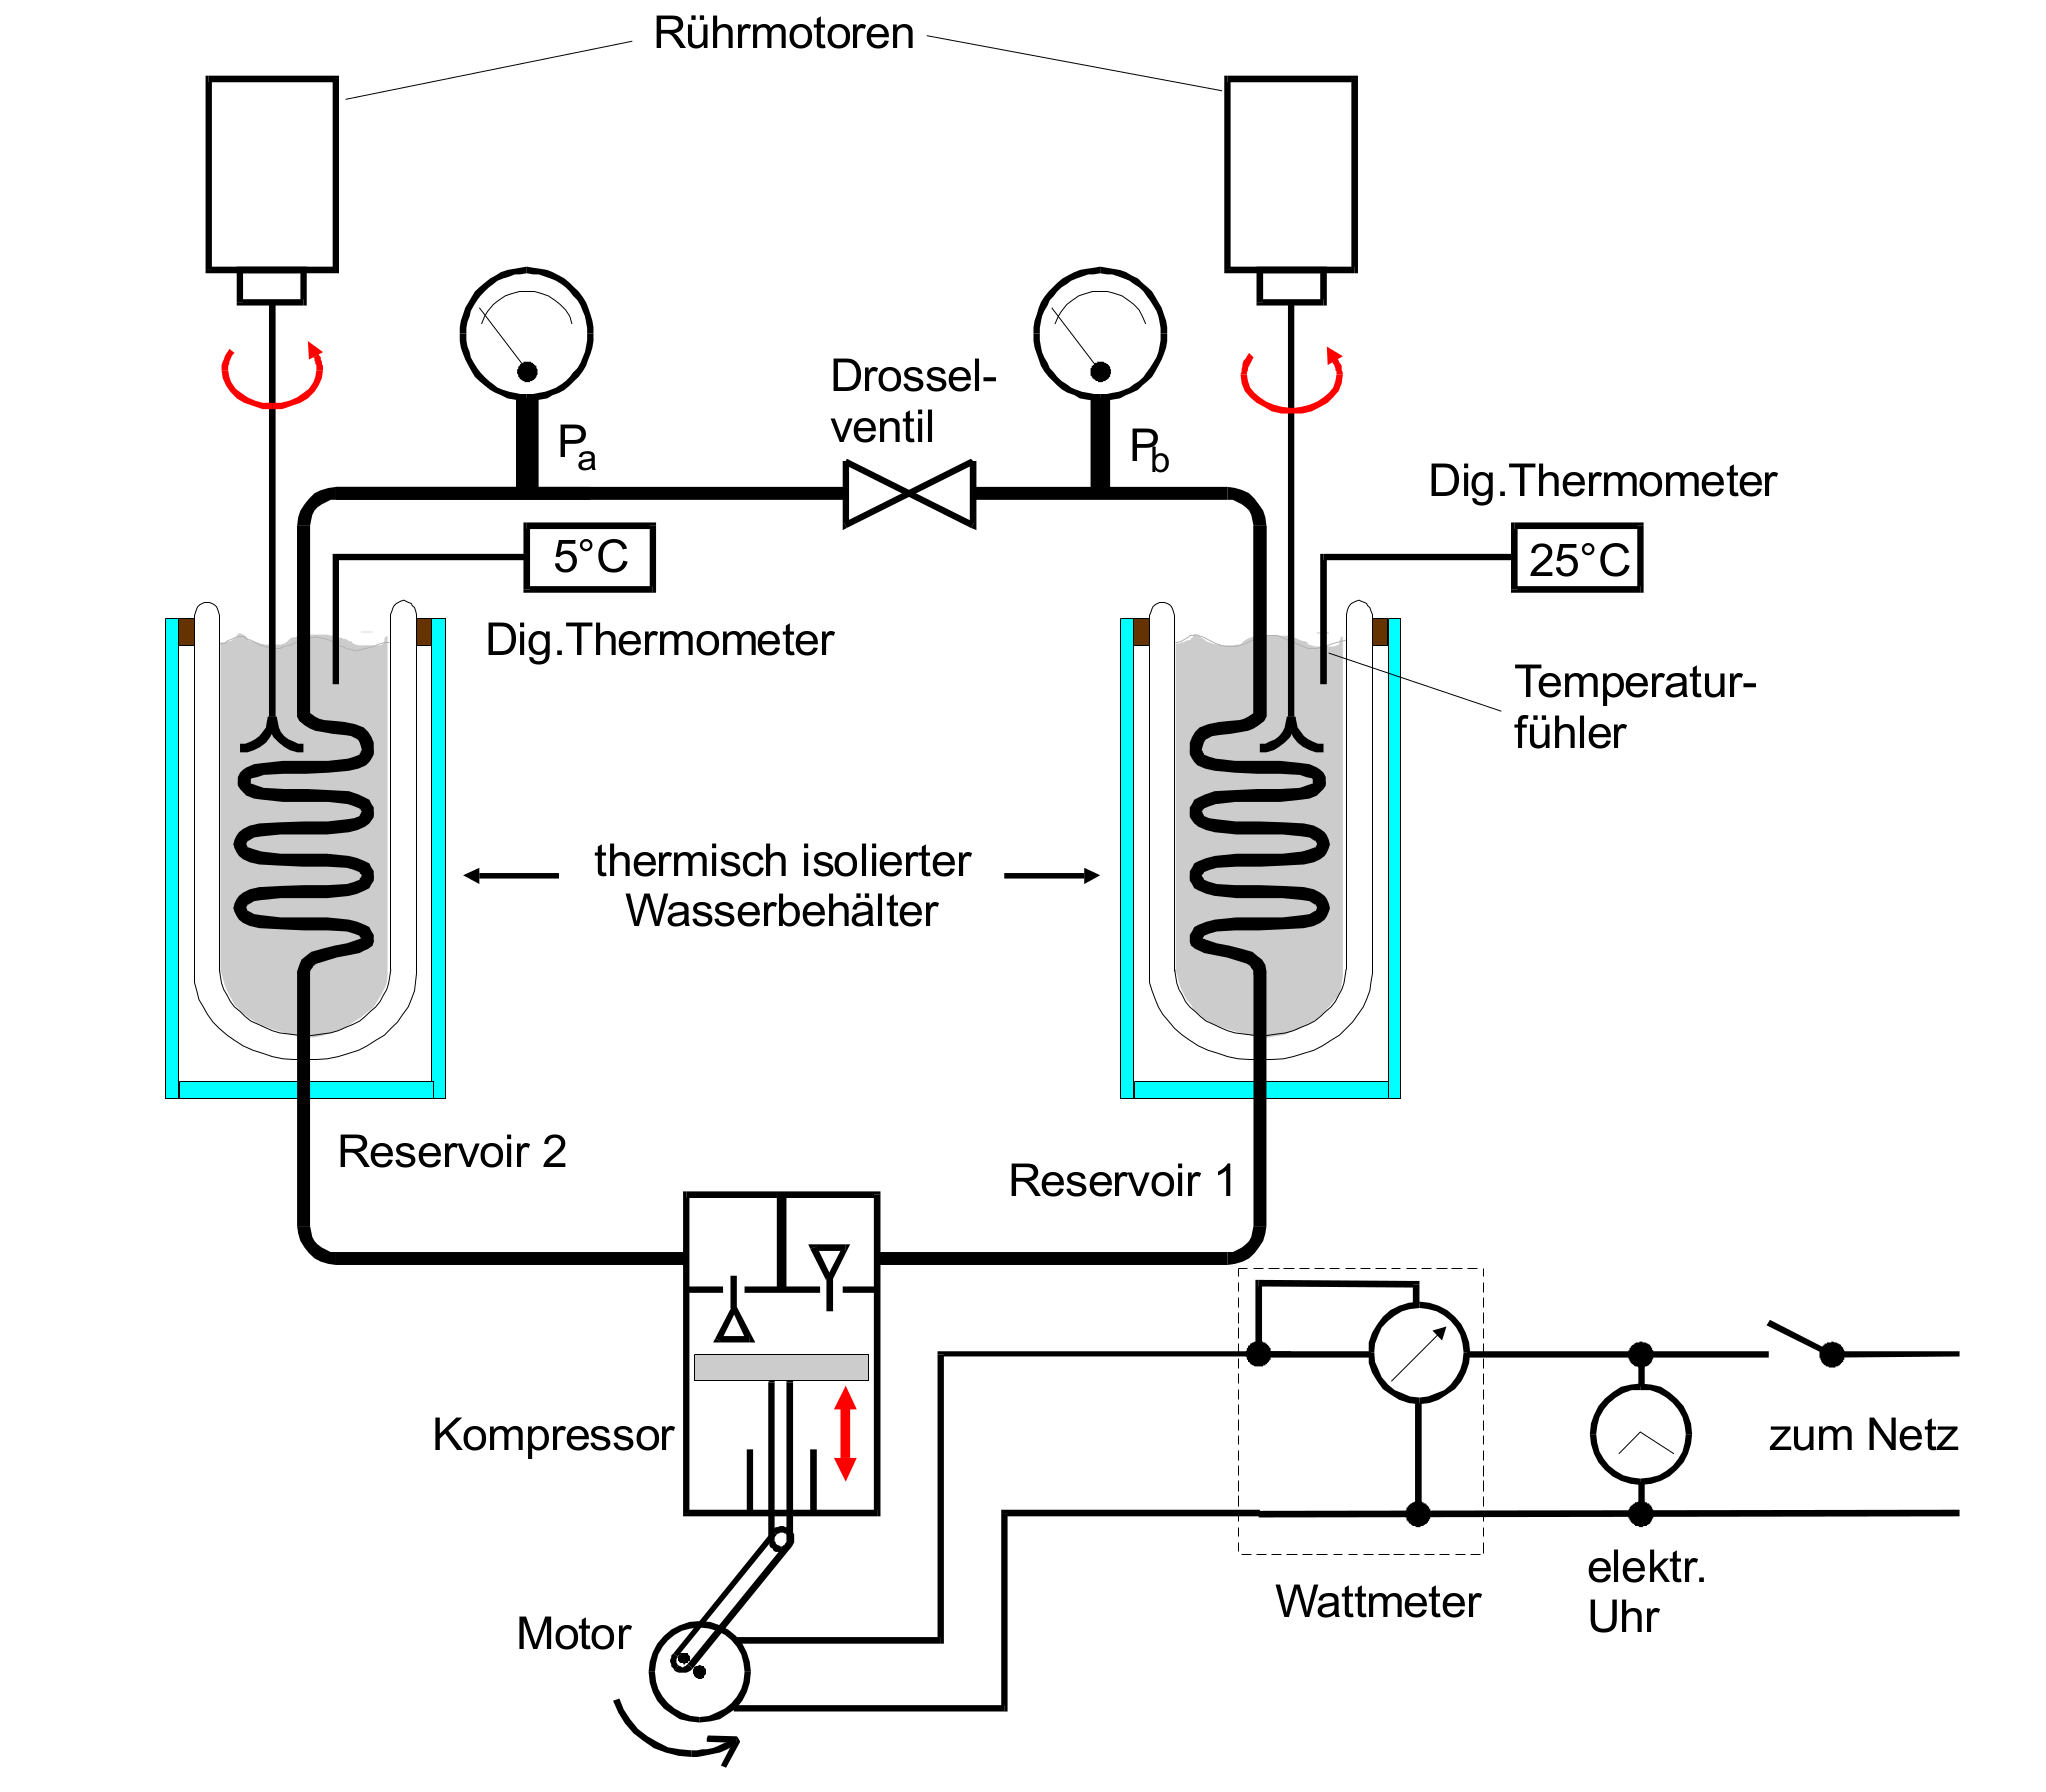
\includegraphics[scale = 0.13]{AufbauMessreihe.png}
        \caption{Die Messapparatur.}
        \label{fig:wärmepumpe2}
      \end{figure}
      In die thermisch isolierten Reservoir 1 und 2 wird eine genau abgemessene Menge kaltes Wasser gefüllt. Damit eine zuverlässige Temperaturmessung mithilfe der beiden
      Digitalthermometer stattfinden kann, werden die Reservoire mit den Rührmotoren während des Experiments laufend durchgerührt. Die Drücke $p_\text{2}$ und $p_\text{1}$
      vor und hinter dem Drosselventil und die Leistungsaufnahme des Kompressors werden ebenfalls aufgenommen. Alle Messwerte werden in Abhängigkeit der Zeit gemessen.
      Jede Minute wurde eine Messung durchgeführt, bis Reservoir 1 eine Temperatur von $T_\text{1} = \SI{50}{\celsius}$ erreicht hat.
\section{Auswertung der Messdaten}
    Die gemessenen Daten sind in der folgenden Tabelle \ref{tab:Messdaten} dargestellt.
    %Tabelle mit Messdaten in SI

\begin{table}
    \centering
    \caption{Messdaten}
    \label{tab:Messdaten}
    \begin{tabular}{S S S S S S}
        \toprule
        {$t [s]$} & {$T1 [K]$} & {$p1 [Pa]$} & {$T2 [K]$} & {$p2 [Pa]$} & {$N [W]$} \\
        \midrule
        0.00   &      294.85  &   500000.00  &      294.85  &   510000.00  &      120.00 \\
        60.00  &      296.15  &   600000.00  &      294.85  &   420000.00  &      120.00\\
       120.00  &      297.45  &   650000.00  &      294.75  &   440000.00  &      120.00\\
       180.00  &      298.45  &   700000.00  &      294.65  &   450000.00  &      120.00\\
       240.00  &      299.55  &   700000.00  &      293.95  &   450000.00  &      120.00\\
       300.00  &      300.65  &   700000.00  &      293.25  &   440000.00  &      120.00\\
       360.00  &      301.95  &   750000.00  &      292.35  &   430000.00  &      120.00\\
       420.00  &      302.85  &   750000.00  &      291.65  &   420000.00  &      120.00\\
       480.00  &      304.05  &   800000.00  &      290.85  &   420000.00  &      120.00\\
       540.00  &      305.05  &   800000.00  &      290.05  &   400000.00  &      120.00\\
       600.00  &      306.05  &   800000.00  &      289.35  &   400000.00  &      120.00\\
       660.00  &      307.05  &   850000.00  &      288.65  &   390000.00  &      120.00\\
       720.00  &      307.95  &   850000.00  &      288.05  &   380000.00  &      120.00\\
       780.00  &      308.85  &   900000.00  &      287.35  &   380000.00  &      120.00\\
       840.00  &      309.85  &   900000.00  &      286.75  &   370000.00  &      120.00\\
       900.00  &      310.75  &   900000.00  &      286.15  &   360000.00  &      120.00\\
       960.00  &      311.55  &   950000.00  &      285.55  &   360000.00  &      120.00\\
      1020.00  &      312.35  &   950000.00  &      284.85  &   360000.00  &      120.00\\
      1080.00  &      313.15  &  1000000.00  &      284.45  &   350000.00  &      120.00\\
      1140.00  &      313.85  &  1000000.00  &      284.05  &   350000.00  &      120.00\\
      1200.00  &      314.55  &  1000000.00  &      283.55  &   340000.00  &      120.00\\
      1260.00  &      315.35  &  1000000.00  &      283.05  &   340000.00  &      120.00\\
      1320.00  &      316.05  &  1050000.00  &      282.65  &   340000.00  &      120.00\\
      1380.00  &      316.75  &  1050000.00  &      282.25  &   340000.00  &      120.00\\
      1440.00  &      317.45  &  1100000.00  &      281.85  &   340000.00  &      120.00\\
      1500.00  &      318.05  &  1100000.00  &      281.45  &   340000.00  &      120.00\\
      1560.00  &      318.65  &  1100000.00  &      281.15  &   330000.00  &      120.00\\
      1620.00  &      319.25  &  1100000.00  &      280.85  &   320000.00  &      122.00\\
      1680.00  &      319.85  &  1150000.00  &      280.55  &   320000.00  &      122.00\\
      1740.00  &      320.45  &  1150000.00  &      280.25  &   320000.00  &      122.00\\
      1800.00  &      320.95  &  1175000.00  &      279.95  &   320000.00  &      122.00\\
      1860.00  &      321.55  &  1200000.00  &      278.75  &   320000.00  &      122.00\\
      1920.00  &      322.05  &  1200000.00  &      277.45  &   320000.00  &      122.00\\
      1980.00  &      322.55  &  1200000.00  &      276.55  &   320000.00  &      122.00\\
      2040.00  &      323.05  &  1200000.00  &      276.15  &   320000.00  &      122.00\\
      2100.00  &      323.45  &  1200000.00  &      276.05  &   320000.00  &      122.00\\   
        \bottomrule
    \end{tabular}
\end{table}
    %Aufgabenteil a)
\subsection{Temperaturmessung}
Im folgenden Diagramm werden die Verläufe der Temperaturen T1 und T2 in Abhängigkeit der Zeit aufgetragen.
Alle Werte wurden in SI-Einheiten konvertiert.
\begin{figure}
  \centering
  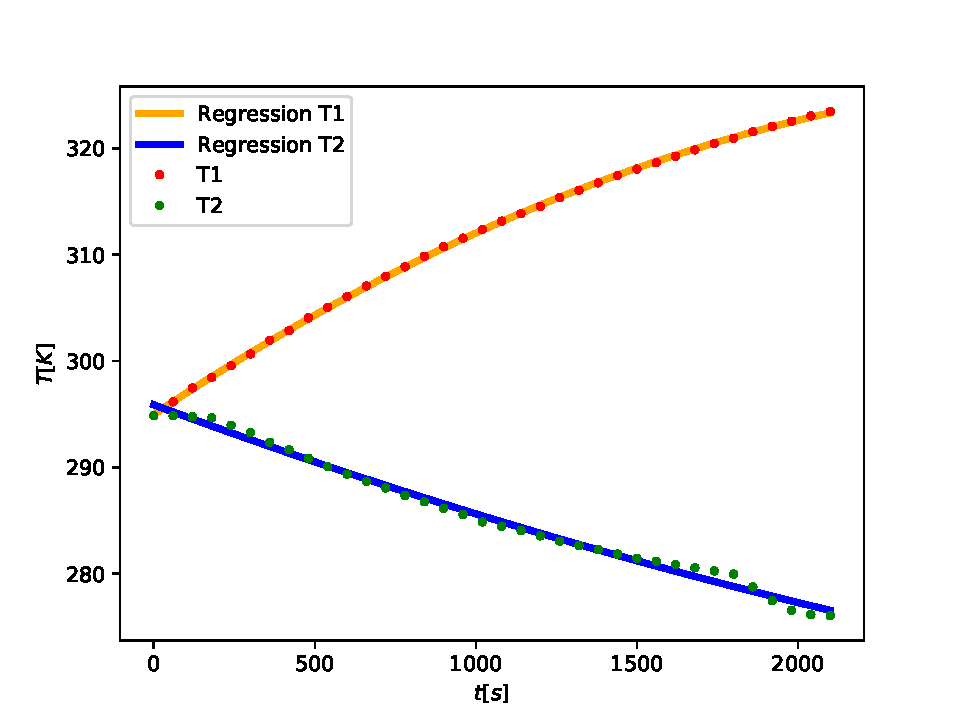
\includegraphics[scale = 0.75]{Temperaturverlaeufe.pdf}
  \caption{Die beiden Temperaturverläufe der Reservoire 1 und 2.}
  \label{fig:TemperaturverlaufA}
\end{figure}

%Aufgabenteil b)
\subsection{Bestimmung der Näherungsfunktion}
Die quadratische Regression ist ebenfalls in \ref{fig:TemperaturverlaufA} skizziert. Der gewählte Ansatz ist
\begin{equation}
  T(t) = \symup{A} \cdot t^2 + \symup{B} \cdot t + \symup{C}.
  \label{eq:Regressionsgleichung}
\end{equation}
\begin{table}
  \centering
  \caption{Parameter der quadratischen Regression}
  \label{tab:regression1}
  \sisetup{table-format=3.7}
  \begin{tabular}{c S S S S S S}
    \toprule
     {$T$} & {$A [\mu K/s^2]$} & {$\increment A [nK/s^2]$} & {$B [mK/s]$} & {$\increment B [\mu K/s]$} & {$C [K]$} & {$\increment C [K]$} \\
    \midrule
    {$T_\text{1}$} & -3.22492 &  41.934 &  20.27984 & 91.1047 & 294.97008 & 0.04134 \\
    {$T_\text{2}$} & 0.95504 &  267.11 & -11.20871 & 580.316 & 295.87019 & 0.26336 \\
    \bottomrule
  \end{tabular}
\end{table}

%Aufgabenteil c)
\subsection{Bestimmung der Differentialquotienten}
Die Differentialquotienten der Regressionen berechnet man durch einfaches Ableiten der Gleichung \eqref{eq:Regressionsgleichung}.
Nach den Ableitungsregeln ergibt sich:
\begin{equation}
    T'(t) = 2\symup{A} \cdot t + \symup{B}
    \label{eq:Regressionableitung}
\end{equation}
  Nun werden konkrete Werte für 4 verschiedene Temperaturen berechnet werden. Diese sind in unserem Fall die Temperaturen bei 
  den Zeiten $60s, 660s, 1 260s, 1 860s$.
  \begin{table}
    \centering
    \caption{Differentialquotienten}
    \label{tab:Differentialquotienten}
    \sisetup{table-format=1.5}
    \begin{tabular}{c S S S S S S}
      \toprule
       {$t [s]$} & {$T_{1}'(t) [K/s]$} & {$\increment T_{1}'(t) [\mu K/s]$} & {$T_{2}'(t) [K/s]$} & {$\increment T_{2}'(t) [mK/s]$} \\
      \midrule
      60 & 0.02027 & 91.1047 & 0.01121 & 0.580316 \\
      660 & 0.02020 & 91.1047 & 0.01118 & 0.580345 \\
      1260 & 0.02014 & 91.1216 & 0.01117 & 0.580424 \\
      1860 & 0.02007 & 91.1417 & 0.01115 & 0.580552 \\
      \bottomrule
    \end{tabular}
  \end{table}

\subsection{Bestimmung der Güteziffer}
Mithilfe der Differentialquotienten soll mit \eqref{eqn:realegüteziffer3} die reale Güteziffer berechnet werden. Zudem soll diese mit der
idealen Güteziffer verglichen werden, die mit \eqref{eqn:idealegüteziffer} berechnet wird. 
Die Abweichung p der Beiden Werte in Prozent wird berechnet mit:
\begin{equation}
  p=\frac{v_{id}-v_{real}}{v_{id}} \cdot 100
\end{equation}
Die Berechnung bei den vier oben beschriebenen
Zeitpunkten ergibt: 
\begin{table}
  \centering
  \caption{Güteziffern für T1}
  \label{tab:gütezifferT1}
  \sisetup{table-format=1.5}
  \begin{tabular}{S[table-format=4.1] S S S[table-format=3.0] S[table-format=2.5] S}
    \toprule
    {$t [s]$} & {$v_{real1}$} & {$\increment v_{real1}$} & {$v_{id1}$} & {$p_1$} & {$\increment p_1$} \\
    \midrule
    60 & 2.95349 & 0.01327 & 227 & 98.70351 & 0.00583 \\
    660 & 2.94409 & 0.01327 & 16 & 82.35746 & 0.07954 \\
    1260 & 2.93470 & 0.01327 & 9 & 69.94106 & 0.13597 \\
    1860 & 2.87735 & 0.01306 & 7 & 61.70096 & 0.17384 \\
      \bottomrule
  \end{tabular}
\end{table}

\begin{table}
\centering
\centering
  \caption{Güteziffern für T2}
  \label{tab:gütezifferT2}
  \sisetup{table-format=1.5}
  \begin{tabular}{S[table-format=4.0] S S S[table-format=3.0] S[table-format=2.5] S}
    \toprule
     {$t [s]$} & {$v_{real2}$} & {$\increment v_{real2}$} & {$v_{id2}$} & {$p_2$} & {$\increment p_2$} \\
    \midrule
    60 & 1.63264 & 0.08454 & 226 & 99.28016 & 0.03727 \\
    660 & 1.62986 & 0.08454 & 15 & 89.61044 & 0.53894 \\
    1260 & 1.62707 & 0.08456 & 8 & 69.94105 & 0.96492 \\
    1860 & 1.59767 & 0.08319 & 6 & 75.46897 & 1.27773 \\
      \bottomrule
  \end{tabular}
\end{table}

Es fällt auf, dass die Abweichung der realen Güteziffer von dem idealen Wert stark abweicht. 
Mögliche Gründe für diese Abweichung werden in \ref{sec:Auswertung} angegeben.

\subsection{Bestimmung des Massendurchsatzes}
Die Berechnung des Massendurchsatzes erfolgt mit \eqref{eqn:massendurchsatz2}. Dafür muss aber zuerst die 
Verdampfungswärme L bestimmt werden. 
\\
Aus V203-"Verdampfungswärme" ist folgender Zusammenhang zwischen dem Druck p, der Temperatur T, und L bekannt:
\begin{equation}
  ln(p/p_0)=\frac{-L}{R \cdot T}
\end{equation}
$R$ entspricht hierbei der universellen Gaskonstante und $p_0$ entspricht der Umgebungsdruck.
Wählt man nun $x=1/T$ und $y=ln(p-p_0)$, dann erhält man die lineare Gleichung:
\begin{equation}
  y=-\frac{L}{R}\cdot x+c \label{Dampfdruckgleichung}
\end{equation}
Trägt man die Messwerte in ein Koordinaten System ein und setzt wie oben beschrieben $x=1/T$ und $y=ln(p-p_0)$,
wird dieser Zusammenhang gut ersichtlich.
\begin{figure}
  \centering
  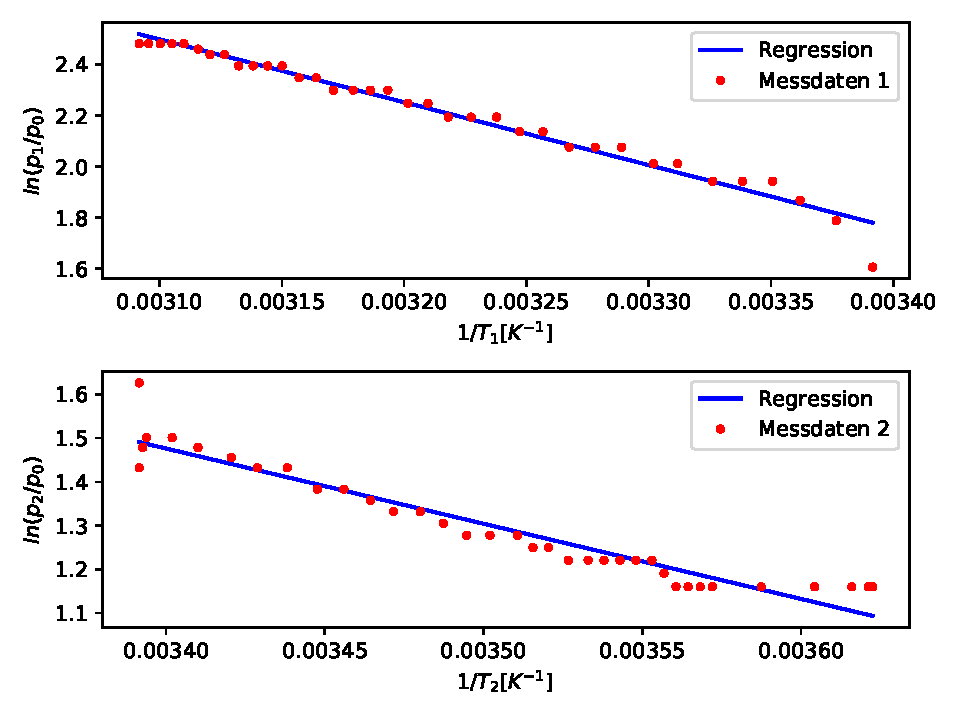
\includegraphics[scale = 0.75]{Druckverlaeufe.pdf}
  \caption{Dampfdruckkurve}
  \label{fig:Dampfdruckkurve}
\end{figure}
Die eingezeichnete Regression hat nun genau die Funktionsgleichung \eqref{Dampfdruckgleichung}. Die Steigung der 
Gerade ist demnach $m=-L/R$. L erhält also durch $L=-m\cdot R$. Durch Einsetzen folgt:
\\
$L=\SI{14299.459 \pm 734.742}{\joule\second\kelvin\per\mole}$
\\
Mit \eqref{eqn:massendurchsatz2} kann man jetzt für die vier verschiedenen Zeiten den Massendurchsatz errechnen:
\begin{table}
  \centering
  \caption{Massendurchsatz}
  \label{tab:massendurchsatz}
  \sisetup{table-format=1.5}
  \begin{tabular}{S[table-format=4.0] S S S S}
    \toprule
    {$t [s]$} & {$\frac{dm}{dt} [mol/s]$} & {$\increment\frac{dm}{dt}[mol/s]$} & {$\frac{dm}{dt} [g/s]$} & {$\increment\frac{dm}{dt}[g/s]$} \\
    \midrule
    60 & 0.01370 & 0.00100 & 1.65659 & 0.12084 \\
    660 & 0.01365 & 0.00100 & 1.65377 & 0.12075 \\
    1 260 & 0.01365 & 0.00100 & 1.65095 & 0.12065 \\
    1 860 & 0.01363 & 0.00100 & 1.64812 & 0.12057 \\
    \bottomrule
  \end{tabular}
\end{table}
Der Massendurchsatz wird in \ref{tab:massendurchsatz} sowohl in $\si{\mole\per\second}$, als auch in $\si{\gram\per\second}$ angegeben.
Man erreicht die Umrechnung mit:
\begin{equation}
  m=M\cdot n
\end{equation}
Hierbei ist $M$ die Molmasse des Gases Dichlordifluormethan $M_{CCl_{2}F_{2}}=\SIlist{120.9}{\kilogram\per\mole}$.

\subsection{Bestimmung der mechanischen Kompressorleistung}
Die mechanische Kompressorleistung $N_{mech}$ wird mit \eqref{eqn:leistungkompressor2} berechnet.
Dabei gilt:
\begin{equation}
  \frac{dV_2}{dt}=\frac{1}{\rho}\frac{dm}{dt} \label{Volumenänderung}
\end{equation}
Das $\rho$ hierbei die Dichte des Gases in Abhängigkeit der Temperatur und des Drucks.
Die Dichte kann man nun mit dem idealen Gasgesetz
\begin{equation}
  pV=nRT \Leftrightarrow \frac{pV}{T}=nR
\end{equation}
berechnen. Da die Stoffmenge $n$ des Gases immer konstant ist, da kein Gas entweicht oder zugeführt wird, und auch
$R$ eine Konstante ist, ist die ganze Rechte Seite konstant. Diese Seite ist für die Temperatur $T_2$, den Druck $p_2$ und das
Volumen $V_2$ gleich den Werten, bei denen die Dichte $\rho_0=\SI{5.514}{\gram\per\liter}$ des Gases gemessen wurde. Diese lauten
$p_0=\SI{e5}{\pascal}$ und $T_0=\SI{273.15}{\kelvin}$.
\begin{equation}
  \frac{p_2V_2}{T_2}=\frac{p_0V_0}{T_0} \Leftrightarrow \frac{p_2m}{\rho_2T_2}=\frac{p_0m}{\rho_0T_0}
\end{equation}
Da die auch die Masse des Gases konstant ist, kann diese herraus gekürzt werden.
Umstellen nach $\rho_2=\rho$ ergibt:
\begin{equation}
  \rho=\frac{\rho_0T_0p_1}{T_2p_0} \label{rho}
\end{equation}
\\
Mit \eqref{rho} und \eqref{Volumenänderung} kann \eqref{eqn:leistungkompressor2} geschrieben werden als:
\begin{equation}
  N_\text{mech} = \frac{1}{\kappa - 1}  \left(p_\text{b} \sqrt[\kappa]{\frac{p_\text{a}}{p_\text{b}}} - p_\text{a} \right)
  \frac{T_2p_0}{\rho_0T_0p_a}\frac{dm}{dt}
\end{equation}
Die mechanische Leistung des Kompressors ist nach Einsetzen der vier ausgewählten Zeiten:
\begin{table}
  \centering
  \caption{mechanische Kompressorleistung}
  \label{tab:kompressorleistung}
  \sisetup{table-format=1.5}
\begin{tabular}{S[table-format=4.0] S[table-format=2.5] S S[table-format=2.5] S}
  \toprule
  {$t [s]$} & {$N_\text{mech} [W]$} & {$\increment N_\text{mech} [W]$} & {$\rho [kg/m^3]$} & {$\increment\rho [kg/m^3]$} \\
  \midrule
  60 & 18.02604 & 0.92977 & 30.53529 & 0.01356\\
  660 & 37.45139 & 1.93178 & 44.18748 & 0.01530\\
  1 260 & 49.78378 & 2.56797 & 53.01378 & 0.01873\\
  1 860 & 59.01109 & 3.04402 & 64.59788 & 0.02317\\
  \bottomrule
\end{tabular}
\end{table}
    \section{Berechnung von Messunsicherheiten}
    \subsection{Berechnung des Mittelwerts}
  \label{sec:mittelwert}
  Für den Mittelwert gilt
  \begin{equation}
    \bar{x}_\text{k} = \frac{1}{N} \sum_{k = 1}^{N} x_\text{k}.
  \end{equation}
\subsection{Berechnung der Standardabweichung}
  \label{sec:standardabweichung}
  Die Standardabweichung berechnet sich wie folgt:
  \begin{equation}
    \increment \bar{x} = \sqrt{\frac{1}{N(N-1)} \sum_{k = 1}^{N}(x_\text{k} - \bar{x})^2 }
  \end{equation}
  mit Messwerten $x_\text{k}$ mit zufälligem Fehler.
\subsection{Fehlerfortpflanzung nach Gauß}
  \label{sec:fehlerfortpflanzung}
  Für $n$ Messgrößen $n_\text{1}$, $n_\text{2}$, ..., $n_\text{N}$ mit der Unsicherheit
  $\increment n_\text{1}$, $\increment n_\text{2}$, ..., $\increment n_\text{N}$. Für die Unsicherheit
  der abgeleiteten Größe gilt
  \begin{equation}
    \increment f = \sqrt{\left(\frac{\partial f}{\partial n_\text{1}} \right)^2 (\increment n_\text{1})^2 + \left(\frac{\partial f}{\partial n_\text{2}} \right)^2 (\increment
    n_\text{2})^2 + ... + \left(\frac{\partial
    f}{\partial  n_\text{n}} \right)^2 (\increment  n_\text{n})^2}
  \end{equation}
\subsection{Lineare Regression}
  \label{sec:regression}
  Für ($x_\text{1}$, $y_\text{1} \pm \sigma$), ..., ($x_\text{N}$, $y_\text{N} \pm \sigma$) linear abhängige Größen und der Geradengleichung $y = m \cdot x + b$ ergibt sich die
  Regression zu
  \begin{align}
    \hat{m}  & = \frac{\bar{xy} - \bar{x} \cdot \bar{y}}{\bar{x^2} - \bar{x}^2} \\
    \hat{b}  & = \bar{y} - \hat{m} \bar{x}
  \end{align}
  Für die Unsicherheit $\sigma_\text{m}^2$ und $\sigma_\text{b}^2$ gilt dann
  \begin{align}
    \sigma_\text{m}^2 & = \frac{\sigma^2}{N(\bar{x^2} - \bar{x}^2)} \\
    \sigma_\text{b}^2 & = \frac{\sigma^2 \bar{x^2}}{N(\bar{x^2} - \bar{x}^2)}
  \end{align}

    \section{Diskussion der Ergebnisse}
      \label{sec:Auswertung}
      Es fällt auf, das die errechnete Güteziffer der Wärmepumpe relativ weit von der idealen abweicht, siehe \ref{tab:gütezifferT1} und \ref{tab:gütezifferT2}. Dies liegt vermutlich
      an der Isolierung der
      Reservoire, die einen Wärmeaustausch mit der Umgebung nicht vollständig verhindern kann. Außerdem läuft die Kompression nur annähernd adiabatisch ab, hier treten also weitere
      Verluste auf. Zudem haben wir die Messung nicht selber durchgeführt, möglicherweise ist auch die Genauigkeit der Messung in Zweifel zu ziehen.
\end{document}
